% 1. Hafta 
% -> Neden Python?
% -> Program Introduction
% -> IDE kurulumu
% -> Programlama ve Pythona giriş
% 	- Variables
% 	- Console input output

% created by Uwe Schadewald
% modified by Mathias Kuntze and Ahmet Uysal
% Add, handout to documentclass arguments for condensed pdf
\documentclass[presentation, 8pt, mathserif, t]{beamer} % , aspectratio=169
\usepackage[english]{babel}
\usepackage{pgf,graphicx}
\usepackage{amsmath, amssymb}
\usepackage[utf8]{inputenc}
\usepackage{lmodern}
\usepackage{palatino}
\usepackage{multimedia}
\usepackage{pgfpages} 
\usepackage{tikz}
\usepackage{datetime}
\pdfoptionpdfminorversion=5

\usepackage{caption}
\usepackage{subcaption}
% if else
\usepackage{ifthen}
% extend table options
\usepackage{tabularx} 
\usepackage{booktabs}
\usepackage{multicol}
\usepackage{multirow}
\usepackage{eso-pic}  % package to set background image
\usepackage[calc]{picture}

% Packages and stuff for ToDo list like itempoints
\usepackage{pifont}
\newcommand{\cmark}{\ding{51}}%
\newcommand{\xmark}{\ding{55}}%
\newcommand{\open}{$\square$}
\newcommand{\done}{\rlap{$\square$}{\raisebox{1pt}{\large\hspace{1.5pt}\cmark}}\hspace{-2.5pt}}
\newcommand{\wontfix}{\rlap{$\square$}{\raisebox{1pt}{\large\hspace{1.5pt}\xmark}}}
\newcommand{\notsure}{\rlap{$\square$}{\raisebox{0.8pt}{\large\hspace{1.5pt}\textbf{?}}}}



% side bar and footer
\setbeamertemplate{headline}{	
	\leavevmode
	\vspace{-4em}	
	\hbox{		
		\begin{beamercolorbox}[wd=0.85\paperwidth,ht=10ex,dp=8ex,center]{}%			
			% navigation with subsections as dots
			\hspace{3.5em}\insertnavigation{0.7\paperwidth}{\hskip0pt plus1fill} % add navigation in footer						
			% navigation with sections, no subsections
			% \insertsectionnavigationhorizontal{0.6\paperwidth}{\hskip0pt plus1fill}{} \\ % add navigation in footer}
			
		\end{beamercolorbox} 				
	}
	\vskip0pt
}


\setbeamertemplate{footline}{	
	\leavevmode
	\vspace{-3em}
	\hbox{
		\begin{beamercolorbox}[wd=.33\paperwidth,ht=2.25ex,dp=1ex,left]{author in head/foot}%
			\hspace{5em}
			\insertshortauthor
		\end{beamercolorbox}
		\begin{beamercolorbox}[wd=.33\paperwidth,ht=2.25ex,dp=1ex,center]{title in head/foot}%
			\insertshorttitle \ - \insertshortsubtitle
		\end{beamercolorbox}	
		\begin{beamercolorbox}[wd=0.30\paperwidth,ht=10ex,dp=8ex,right]{pagenumber in head/foot}			 	
			\insertframenumber % add page numbers
		\end{beamercolorbox}
	}			
	\vskip0pt
}



\setbeamertemplate{frametitle}{
	\ifthenelse{\equal{\insertframesubtitle}{}}{
		\vspace{0.6cm}
		\huge{\insertframetitle}
	}{
		\vspace{0.6cm}
		\small{\insertframetitle}\\
		\vspace{0.3cm}
		\huge{\insertframesubtitle}
    }		
}

	
% enumerate sections
\setbeamertemplate{section in head/foot}{\hfill\insertsectionheadnumber.~\insertsectionhead}
%\setbeamertemplate{section in head/foot shaded}{\color{structure!50}\hfill\insertsectionheadnumber.~\insertsectionhead}
\setbeamertemplate{section in toc}{\inserttocsectionnumber.~\inserttocsection}

%enumerate subsections
\setbeamertemplate{subsection in head/foot}{\hfill\insertsubsectionheadnumber.~\insertsubsectionhead}
\setbeamertemplate{subsection in head/foot shaded}{\color{structure!50}\hfill\insertsubsectionheadnumber.~\insertsubsectionhead}
%\setbeamertemplate{subsection in toc}[subsections numbered]
\setbeamertemplate{subsection in toc}{\vskip0.5em\leftskip=2em\inserttocsubsection\par}

%--------------------------Common------------------------------------------------------
\setbeamercovered{transparent} % make the beamer theme invisible
\usefonttheme{structurebold}
\beamertemplatenavigationsymbolsempty % set navigations helper function to off
\setbeamertemplate{bibliography item}[text]
\setbeamertemplate{note page}[plain]

%\setlist[itemize,1]{label={$\bullet$}} % \item are using bullets
\setbeamertemplate{itemize items}[circle]
	
	

	
% create a new command to show it on two screens
% I'm using dspdfviewer.
\newcommand{\setDualView} {
	\setbeameroption{show notes on second screen=right}
}

%\AtBeginSection[]{\subsection{}}
\newcommand{\addcite}[1]{%
	\AddToShipoutPictureFG*{%
		\AtPageLowerLeft{%
			\put(0.90\paperwidth,5em){											
				\tiny{
					\cite{#1} 
				}			
			}
		}
	}	
}

% insert a frame with references -> use bibtex
\newcommand{\insertReferenceFrame}[3]{%
	\section{#1}
	\begin{frame}[allowframebreaks]
		\frametitle{#1}
		\bibliographystyle{#2}
		\bibliography{#3}
	\end{frame}	
}

\AtBeginSection[]{\subsection{}}
	





\usepackage{../KU-Beamer-Template/style/koc} 
\usepackage{minted}
\usepackage{upquote}
 
\title{KOLT Python} 
\subtitle{Introduction} 
\newdate{date}{18}{02}{2019}
\date{\displaydate{date}}
\author{Ahmet Uysal}

\titlegraphic{
\includegraphics[scale=0.2]{../KU-Beamer-Template/style/images/logo_kolt.eps}}

\setbeamercovered{invisible} % transparent

\begin{document}
  \maketitle

	\frame{\frametitle{Agenda}\tableofcontents}

	\section{Program Information}

	\begin{frame}{Course Outcomes}
		\LARGE
		\begin{itemize}
			\item Apply basic programming concepts using Python
			%\pause
			\item Demonstrate how Python can be used in different areas or disciplines
			%\pause
			\item Create code that is easy to understand
			%\pause
			\item \textbf{Implement practical challenges} by gaining experience in Python
		\end{itemize}
	\end{frame}

	\begin{frame}{Why Python?}
		\vspace{-3mm}
		\inputminted[frame=single,framesep=2pt]{python3}{code-examples/io.py}
		%\pause
		\inputminted[frame=single,framesep=2pt]{java}{code-examples/io.java}
	\end{frame}

	\begin{frame}{Why Python?}
		\begin{itemize}
			\LARGE
			\item Easy Syntax
			\item Beginner Friendly
			-most popular language for introductory CS courses in top universities\cite{guo1}- 
			\item Wide usage area
			\item Large and growing community
		\end{itemize}
	\end{frame}

	\begin{frame}{Some of the Usage Areas\cite{survey_jetbrains2018}}
		\begin{itemize}
			\LARGE
			\item Data Analysis
			%\pause
			\item Web Development
			%\pause
			\item System Administration
			%\pause
			\item Machine Learning
			%\pause
			\item Web Parsers/Scrawlers
			%\pause
			\item Testing
			%\pause
			\item Education
			%\pause
			\item Network Programming
			%\pause
			\item ...
		\end{itemize}	
	\end{frame}
	
	\begin{frame}{Python at Koç University}
		\begin{itemize}
			\LARGE
			\item COMP341: Introduction to Artificial Intelligence
			%\pause
			\item COMP421/521: Introduction to Machine Learning
			%\pause
			\item ENGR350(Selected Topics - Summer18/Spring19): Introduction to Programming for Data Science
			%\pause  
			\item INTL450(Selected Topics - Spring19): Advanced Data Analysis in Python
			%\pause
		\end{itemize}
		\begin{columns}
			\column{0.3\textwidth}
				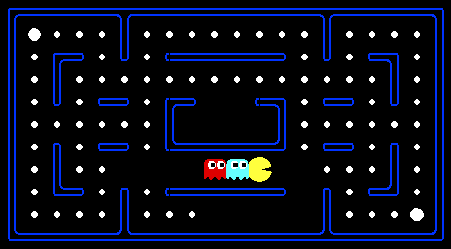
\includegraphics[width=\textwidth]{images/berkeley_pacman.png}
			%\pause
			\column{0.3\textwidth}
				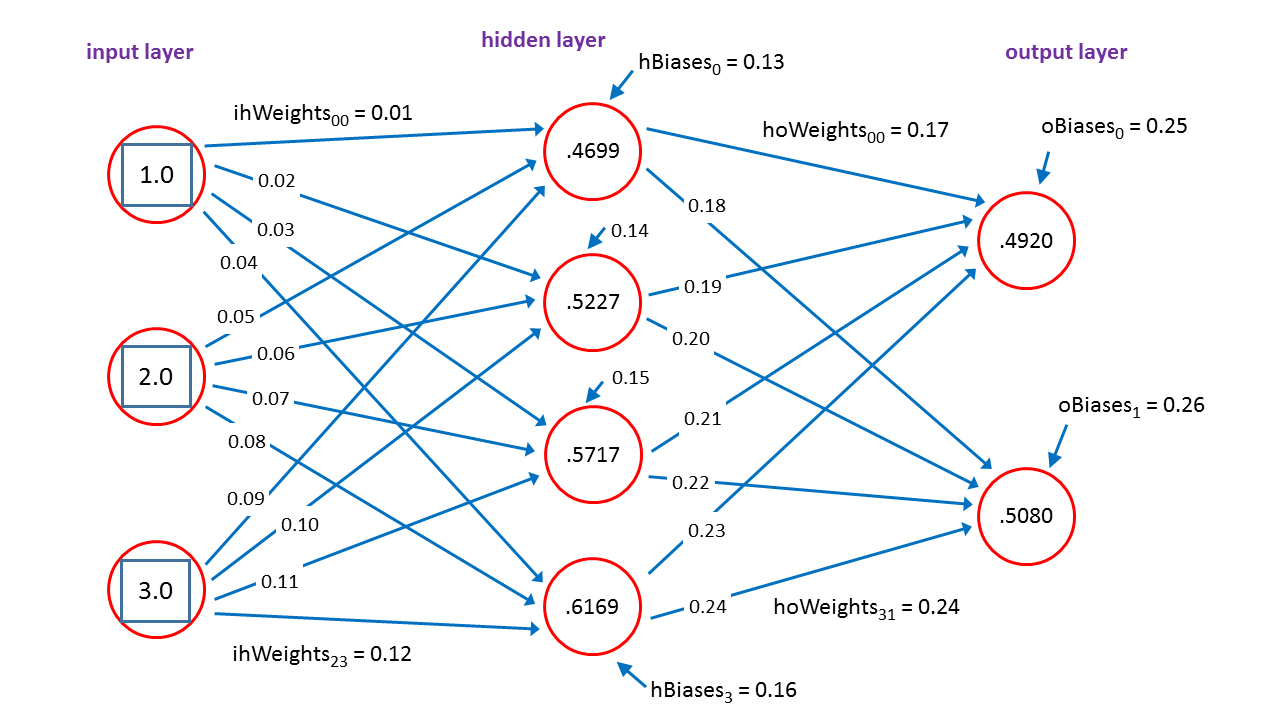
\includegraphics[width=\textwidth]{images/nn.jpg}
			%\pause
			\column{0.3\textwidth}
				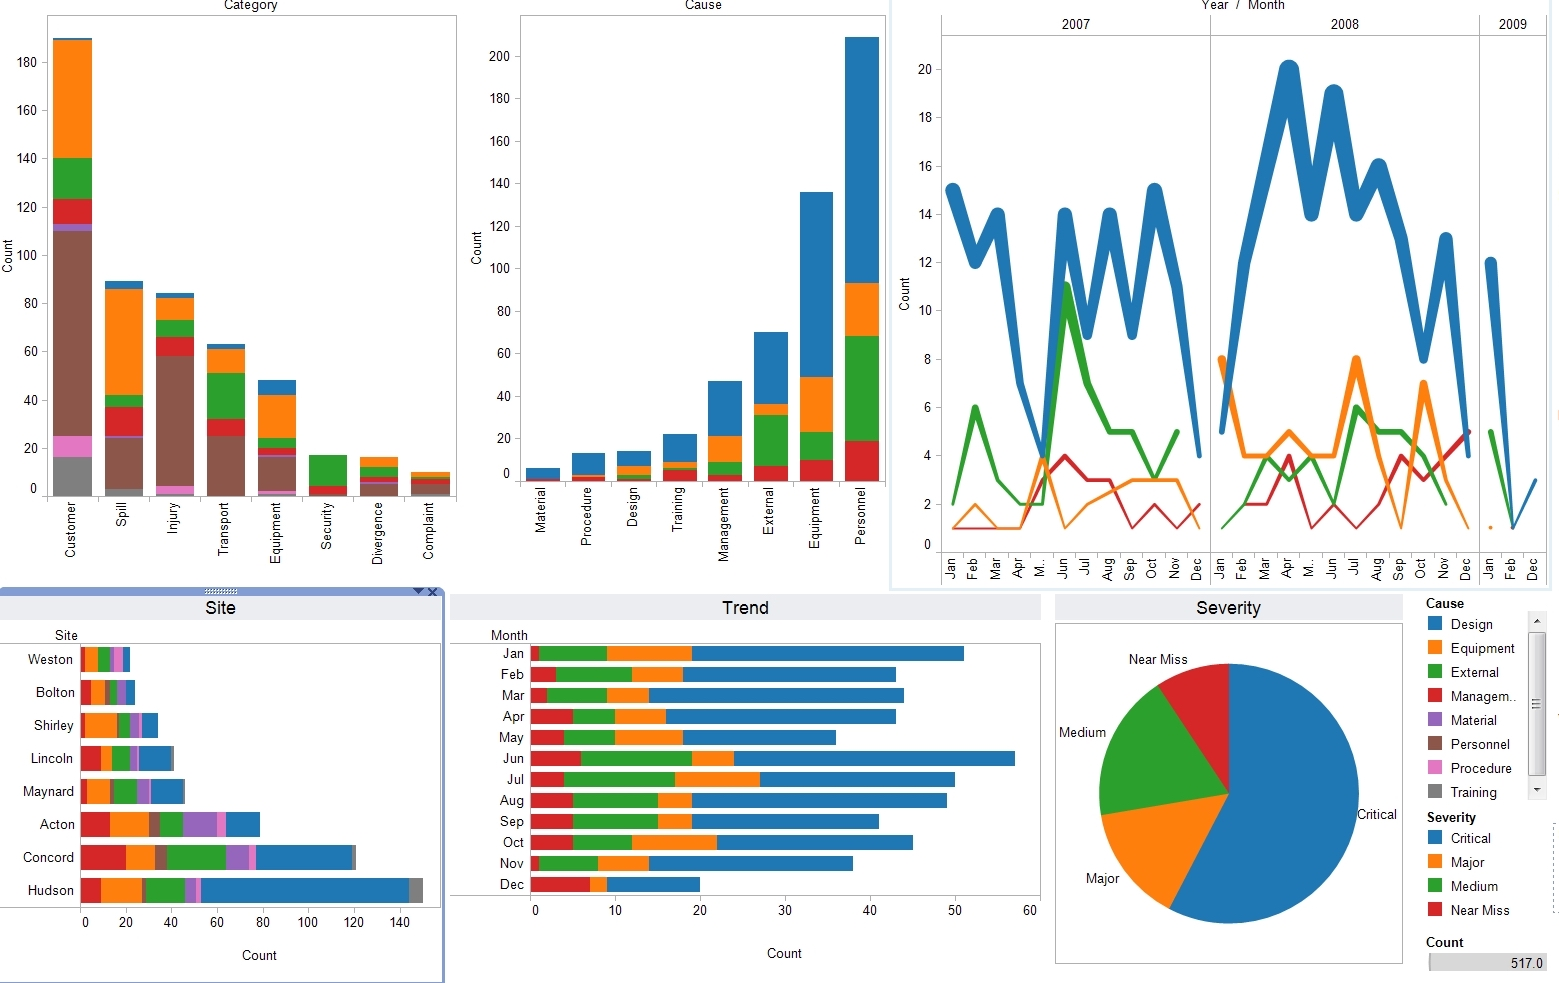
\includegraphics[width=\textwidth]{images/analysis.jpeg}
		\end{columns}
	\end{frame}

	\begin{frame}{Python at Industry}
		\begin{table}[]
			\resizebox{\textwidth}{!}{
			\begin{tabular}{lll}
				
\includegraphics[width=2cm]{images/firefox.png}& 
\includegraphics[width=3cm]{images/google.png} & 
\includegraphics[width=2cm]{images/nasa.png} \\
				
\includegraphics[width=2cm]{images/instagram.png}& 
\includegraphics[width=3cm]{images/youtube.png} & 
\includegraphics[width=2cm]{images/reddit.png}\\
			\end{tabular}}
		\end{table}
	\end{frame}

	\begin{frame}{Python at Industry\cite{instagram_engineering}}
		\centering
		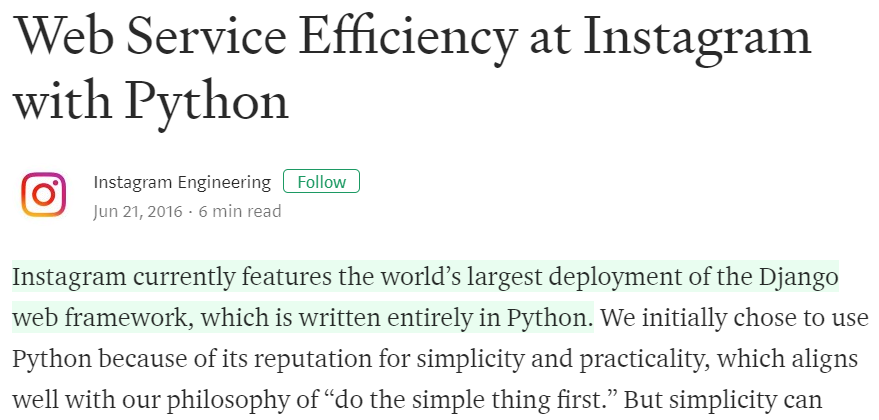
\includegraphics[width=0.6\textwidth]{images/instagram_python.PNG}
		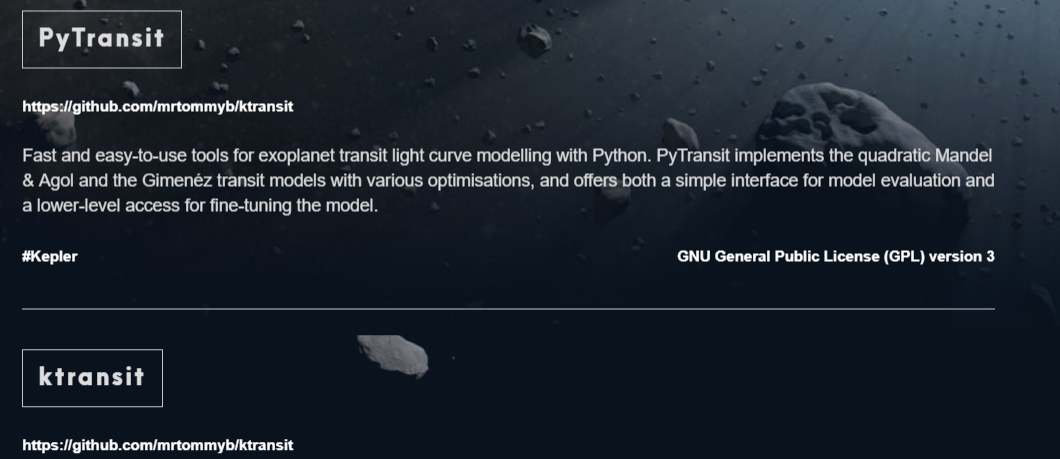
\includegraphics[width=0.6\textwidth]{images/nasa_python.PNG}
	\end{frame}

	\section{Logistics}
		\begin{frame}{Team}
			\begin{columns}
				\column{5cm}
				\centering 
					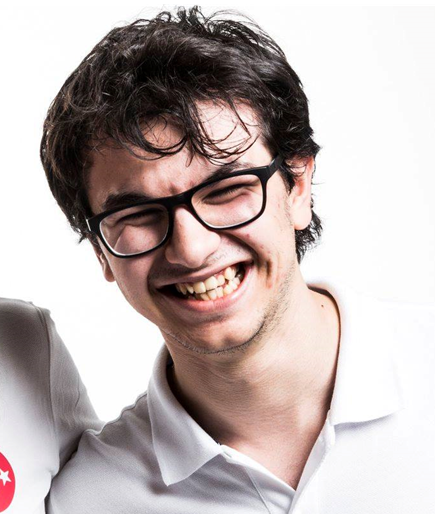
\includegraphics[width=4.0cm]{images/ahmet.png}\\
					Ahmet Uysal\\
					auysal16@ku.edu.tr
				%\pause
				\column{5cm}
				\centering
					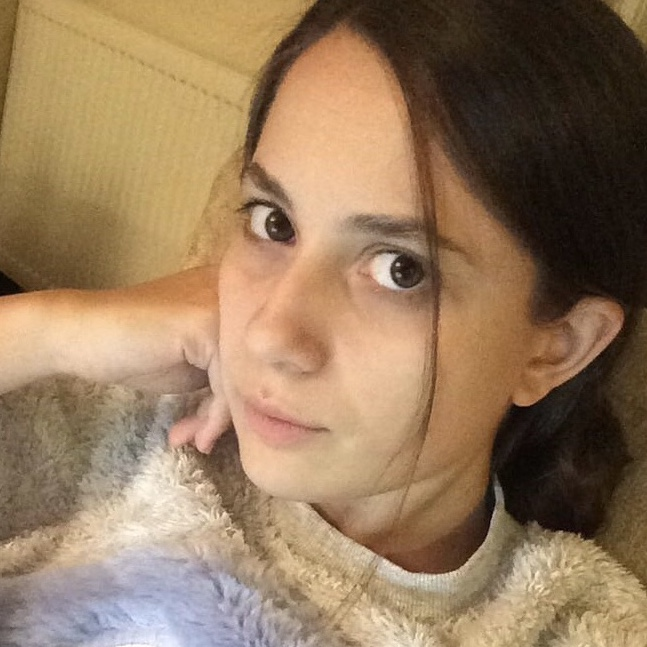
\includegraphics[width=4.0cm]{images/ipek.jpeg}\\
					İpek Köprülülü\\
					ikoprululu16@ku.edu.tr
			\end{columns}
		\end{frame}

		\begin{frame}{Weekly Schedule}
			\LARGE
			\texttt{Monday 17:30-18:45 \textbf{Lecture}}\\
			%\pause
			\texttt{Wednesday 17:30-18:45 \textbf{Contest/Review}}\\
			%\pause  
			\texttt{Every Week \textbf{HackerRank Contest}}\\
			%\pause
			\vspace{4mm}
			\centering
			
\includegraphics[width=6cm]{images/hackerrank.png}\\
			We will use HackerRank a lot this semester, create your account if you have not already!
		\end{frame}

		\begin{frame}{Programming Assignments}
			\begin{itemize}
				\LARGE
				\item 4-6 Programming Assignments
				%\pause
				\item Review sessions will be conducted to \textbf{help you}
				%\pause
				\item Some assignments will have \textbf{autograders} to help you find your mistakes and test your code.
				%\pause
				\item Later assignments will be based on \textbf{your interests!}
				%\pause
				\item We can also organize hackathons if requested :)
			\end{itemize}
			\LARGE
			
		\end{frame}

		\begin{frame}{Programming Contests}
			\begin{itemize}
				\LARGE
				\item Weekly Online Contests
					%\pause
					\begin{itemize}
						\Large
						\item 5-10 Programming questions related to topic we have seen
						%\pause
						\item Duration: 1 week (Starts after the lecture on Monday, ends before next lecture)
						%\pause
						\item First contest will start just after this lecture
					\end{itemize}
				%\pause
				\item Biweekly Onsite Contests
					\begin{itemize}
						\Large
						\item Wednesdays, on weeks which you don't have an assignment
						%\pause
						\item 2-3 Programming questions related to Monday's lecture
						%\pause
						\item Duration: 50 minutes
						%\pause
						\item Questions will be solved in remaining 25 minutes
						%\pause
						\item Surprize gifts to first three places and problem solvers!
					\end{itemize}
			\end{itemize}
		\end{frame}

		\begin{frame}{Certificate Requirements}
			%\pause
			\begin{itemize}
				\LARGE
				\item At most \textbf{3 unexcused absences}, including onsite contests and review sessions.
				%\pause
				\item Working on and submitting all homework assignments. Submissions that do not pass the autograders will be examined by us.
				%\pause
				\item We do not expect that you ace all programming assignments. But, we expect that you \textbf{spend time} on it!
				%\pause
				\item Complying to \href{https://vpaa.ku.edu.tr/academic/student-code-of-conduct}{\underline{\textit{Koç University Code of Conduct}}}. 
			\end{itemize}
		\end{frame}


		\begin{frame}{5 Minute Break}
			\centering
			
\includegraphics[width=\textwidth]{images/you_wordart.PNG}
		\end{frame}

	\section{Installations}

	 	\begin{frame}{Installing Python}
			\LARGE
			\begin{itemize}
				\item Go to \href{https://www.python.org/downloads/}{\underline{\textit{python.org/downloads}}}
				%\pause
				\item Install the Python 3.7.2 for your operating system
				%\pause
				\item (Windows only) Make sure to add python to the \texttt{environment variables} by checking the corresponding permission on the installation or by hand
				%\pause
				\item Check the installation by running \textbf{\texttt{python}}(Windows)/\textbf{\texttt{python3}}(macOS/Linux) in terminal.
			\end{itemize}
			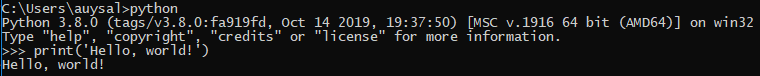
\includegraphics[width=\textwidth]{images/cmd_helloworld.PNG}
		\end{frame}
		 
		\begin{frame}[t]{Installing an Editor/IDE(Integrated Development Environment)}
			\vspace{-4mm}
			\begin{columns}[t] 
				\begin{column}[t]{0.66\linewidth}
					\LARGE
					\begin{itemize}
						\item Although you can edit Python(.py) files with any text editor and run them directly through terminal, having a specialized editor/IDE can help a lot. 
						\item We will use Visual Studio Code in lectures but you are free to use any editor/IDE of your choice.
						\item Get Visual Studio Code from \href{https://code.visualstudio.com/Download}{\underline{\textit{code.visualstudio.com/Download}}}
					\end{itemize}
				\end{column}
				
				\begin{column}{0.33\linewidth}
					\begin{center}
						
\includegraphics[width=0.8\linewidth]{images/vscode.png}						
					\end{center}
				\end{column}
			\end{columns}
	 	\end{frame}

	 	\begin{frame}{Configuring Visual Studio Code for Python}
			\LARGE
			\begin{itemize}
				\item Install Python extension for VS Code.
				%\pause
				\item Select the Python(3.7.2) Interpreter in VS Code.
				%\pause
				\item For more information, visit \href{https://code.visualstudio.com/docs/python/python-tutorial}{\underline{\textit{VS Code Python Tutorial}}}.
			\end{itemize}
			\centering
			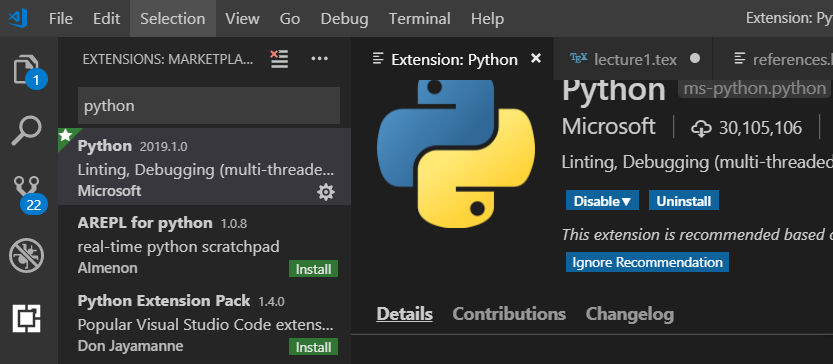
\includegraphics[width=0.75\linewidth]{images/extension_python.PNG}						
	 	\end{frame}

	\section{Introduction}
		\begin{frame}{Interactive Interpreter}
			\LARGE
			You can instantly run code on terminal!
			%\pause
			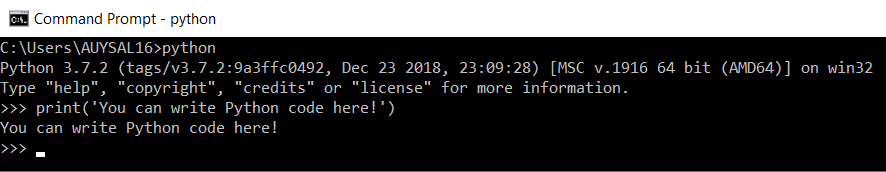
\includegraphics[width=\textwidth]{images/cmd_python.png}
			%\pause
			You can also open a terminal inside VS Code
			\centering
			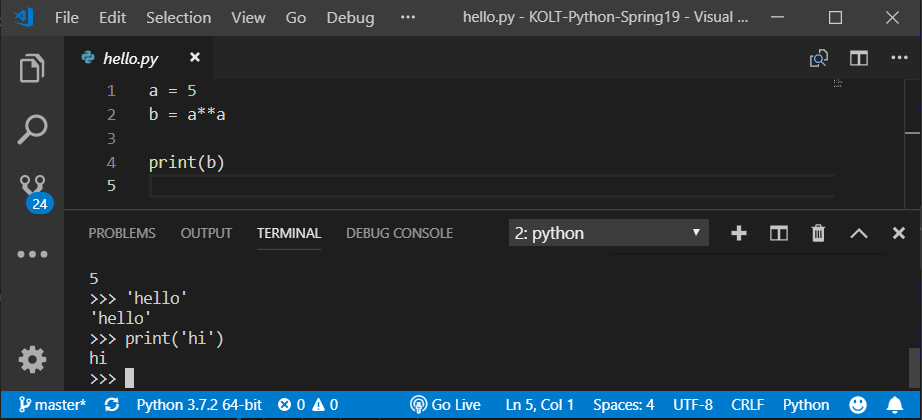
\includegraphics[width=0.5\textwidth]{images/vscode_python.png}
		\end{frame}

		\begin{frame}{Why It Matters?}
			\begin{itemize}
				\LARGE
				%\pause
				\item Immediate gratification :)
				%\pause
				\item Provides a sandboxed environment to experiment
				%\pause
				\item You are not sure what something does, \textbf{try it!}
				%\pause
				\item Shortens code-test-debug cycle and speeds up learning 
			\end{itemize}
		\end{frame}
		
		\begin{frame}{Comments}
			\LARGE
			\inputminted[frame=single,framesep=2pt]{python3}{code-examples/comments.py}
			Python will basically ignore comments, they are purely written \textbf{for humans}!
		\end{frame}

		\begin{frame}{Variables}
			\LARGE
			\begin{itemize}
				\item How to represent/store values in Python?
				%\pause
				\item Which kind of values we need to represent?
				%\pause
					\begin{itemize}
						\Large
						\item Numbers?
						%\pause
						\item Texts?
						%\pause
						\item Individual Characters?
						%\pause
						\item Starting time of the class?
						%\pause
						\item Colors?
						%\pause
						\item Truth Values?
						%\pause
						\item People?
					\end{itemize} 
			\end{itemize}
		\end{frame}

		\begin{frame}{Variables}
			\LARGE
			\begin{table}[]
				\resizebox{\textwidth}{!}{
				\begin{tabular}{|l|l|l|}
				\hline
				\textcolor{koc}{\textbf{Type}} &\textcolor{koc}{\textbf{Explanation}} & \textcolor{koc}{\textbf{Examples}} \\ \hline
				\textbf{\texttt{int}}  & represent \textbf{integers} & 3, 4, 17, -10 \\ \hline 
				\textbf{\texttt{float}} & represent \textbf{real numbers} & 3.0, 1.11, -109.123123 \\ \hline
				\textbf{\texttt{bool}} & represent \textbf{boolean} truth values & \texttt{True}, \texttt{False} \\ \hline
				\textbf{\texttt{str}} & A sequence of characters. & \textquotesingle Hello\textquotesingle, \textquotesingle \textquotesingle, \textquotesingle 3\textquotesingle \\ \hline
				\textbf{\texttt{NoneType}}& special and has one value, None & \texttt{None} \\ \hline
				\end{tabular}}
			\end{table}
			%\pause
			OK, but how do we create one?
		\end{frame}

		\begin{frame}{Variables}
			\inputminted[frame=single,framesep=2pt,fontsize=\LARGE]{python3}{code-examples/variables.py}
		\end{frame}
		
		\begin{frame}{How about type of variables?}
			\LARGE
			Special method called \texttt{\textbf{type()}} 
			\inputminted[frame=single,framesep=2pt]{python3}{code-examples/types.py}
			Python knows variables' type even if you don't know it!
		\end{frame}

		\begin{frame}{Console I/O(Input/Output)}
			\LARGE
			Now we can store the data we know, \\
			%\pause
			how about interacting with user? \\
			%\pause
			\texttt{print(), input()}
			%\pause
			\inputminted[frame=single,framesep=2pt]{python3}{code-examples/io.py}
		\end{frame}

		\begin{frame}{Console I/O(Input/Output)}
			\huge
			\textbf{\texttt{print(*args, sep=\textquotesingle \ \textquotesingle, end=\textquotesingle \textbackslash n\textquotesingle )}}
			%\pause
			\begin{itemize}
				\LARGE
				\item Can take arbitrary number of arguments
				%\pause
				\item Separates elements with space by default
				%\pause
				\item Adds newline character \texttt{\textquotesingle \textbackslash n\textquotesingle} to end by default
			\end{itemize}
			
			%\pause
			\textbf{\texttt{input([prompt])}}
			%\pause
			\begin{itemize}
				\LARGE
				\item Prints the prompt to Console
				%\pause
				\item Program is paused until user enters something
				%\pause
				\item \textbf{returns an \texttt{str} object!} 
			\end{itemize}
		\end{frame}

		\begin{frame}{Example Program}
			\inputminted[frame=single,framesep=2pt,fontsize=\LARGE]{python3}{code-examples/example_io.py}
			%\pause
			\centering
			\vspace{1cm}
			\Huge
			\textbf{LET'S TRY!!!}
		\end{frame}

\section{References}
	\begin{frame}{References}
		\bibliographystyle{IEEETran}
		\bibliography{references}
	\end{frame}

\end{document}